%!TEX root=document.tex

\section{{\large \SeeDB\ } Architecture}
\label{sec:system_architecture}

%In this section, we present an overview of the \SeeDB\ architecture.
% Given an input query on a dataset, the goal of \SeeDB is to recommend
% visualizations the analyst would find most valuable.
% \SeeDB recommends visualizations that the analyst would find most valuable,
% taking into account aspects such as the background, user preferences,
% and context (as discussed in Section~\ref{sec:general-metric}).
\SeeDB is implemented as a middleware layer that can run on
top of any SQL-compliant database system. 
We packaged \SeeDB as a recommendation plugin that can
be incorporated into a visualization tool such as Tableau or Spotfire. 
% As such, \SeeDB\ would ideally be used as a plug-in for existing 
% visualization software.
For evaluating our system, we have combined \SeeDB with a simple visualization
builder interface inspired by Polaris~\cite{polaris}.
Figure \ref{fig:frontend} shows the web frontend for \SeeDB which is composed
of four parts:
(A) dataset selector used to
connect to a database and query a specific table; (B) query builder used to
formulate queries using a form-based interface; (C) visualization builder
used to manually specify visualizations; and (D) \SeeDB recommendations plugin
that displays recommended visualizations.
Recommendations provided by \SeeDB change in response to changes in the query (B)
issued against the database.
We note that the {\em mixed-initiative} design of \SeeDB incorporating both manual
visualization specification and automated recommendations, reflects the
human-in-the-loop philosophy underlying \SeeDB.
We seek to speed up the analytics process not by completely automating the task, but
by providing the analyst real-time support while letting him or her drive the process.
% We seek to support the analytics process while letting the analyst be in the 
% driver's seat. \mpv{Fix sentence.}

\begin{figure}[htb]
\vspace{-10pt}
\centerline{
\hbox{\resizebox{7cm}{!}{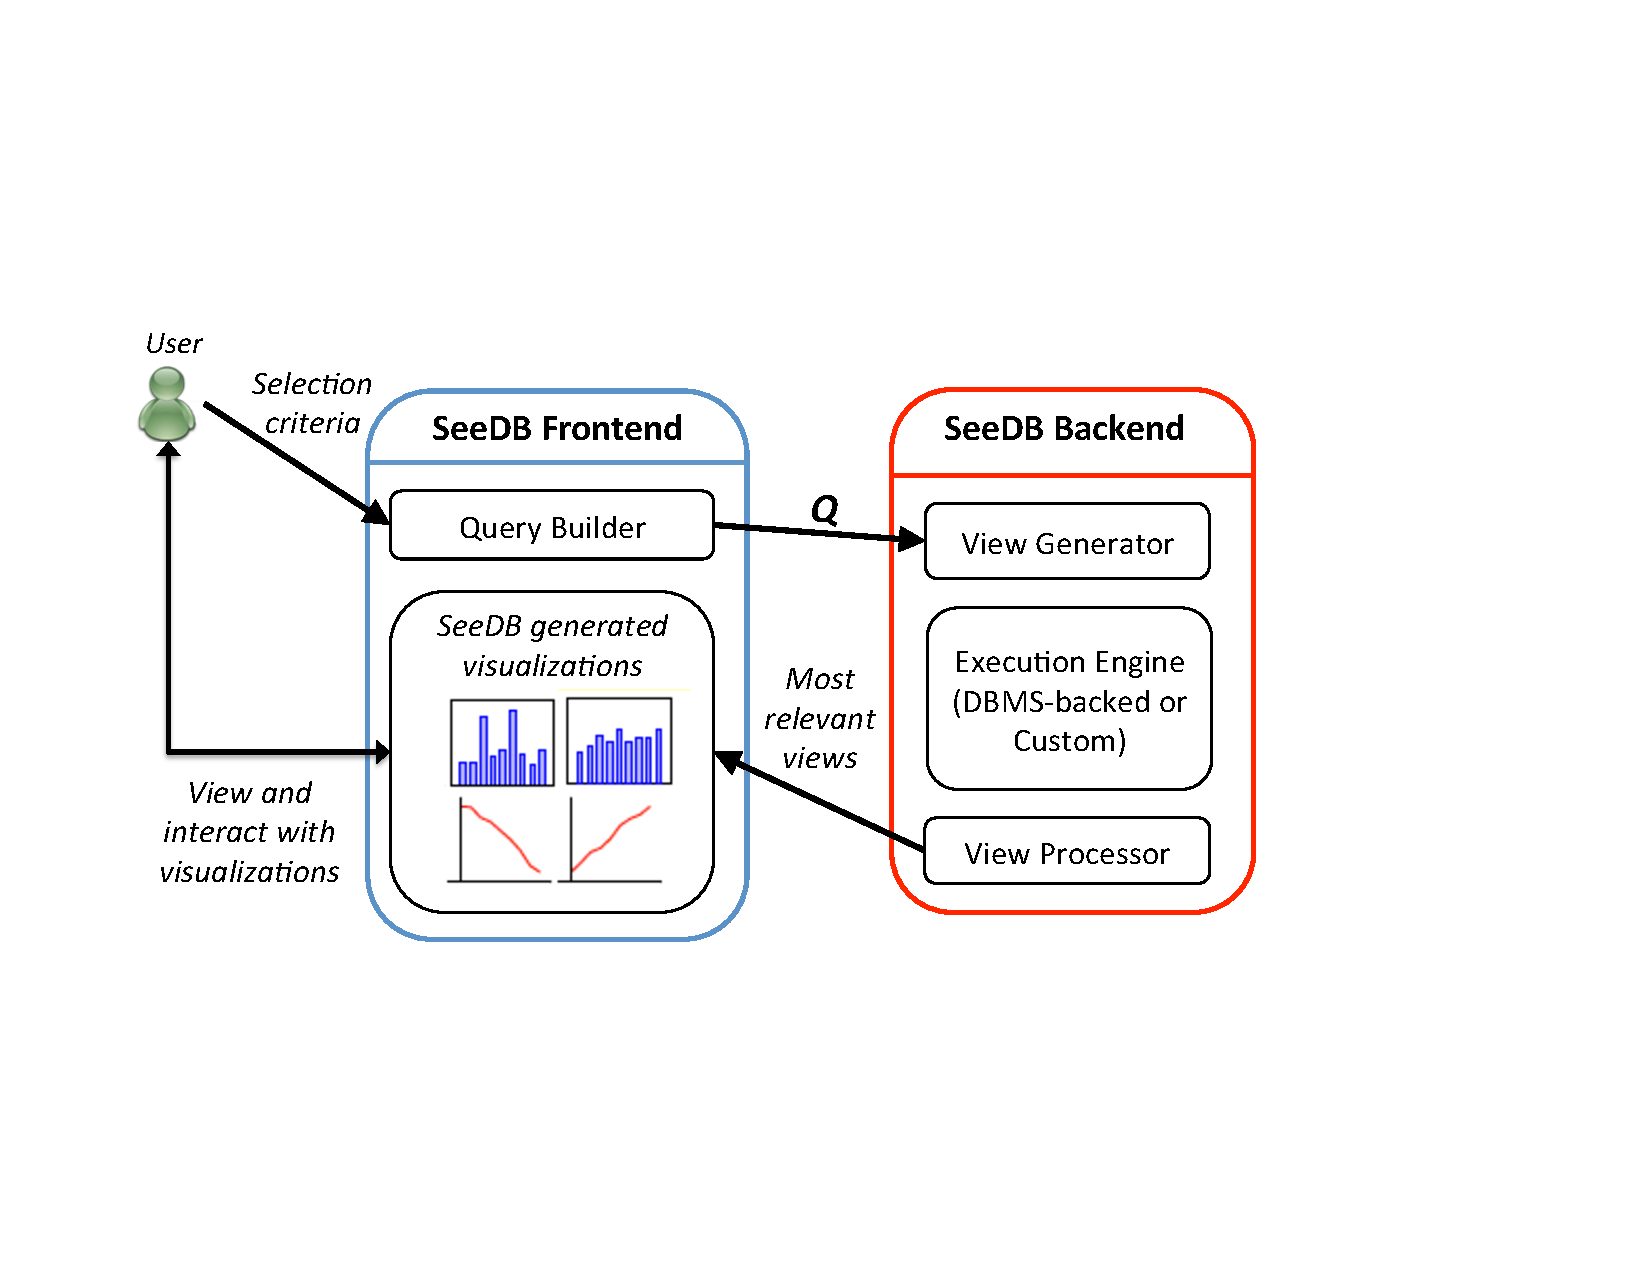
\includegraphics[trim=20mm 45mm 30mm 55mm, 
clip=true]{Images/seedb-architecture.pdf}}}}
\vspace{-18pt}
\caption{SeeDB Architecture}
\label{fig:sys-arch}
\vspace{-12pt}
\end{figure} 
\mpv{Update arch diagram}

The web frontend of \SeeDB is a light-weight client that captures user input and renders
visualizations produced by the backend.
The computational heavy lifting is performed by the \SeeDB server.
Figure \ref{fig:sys-arch} depicts the overall architecture of our system.
The \SeeDB backend is composed of four main components.
The first component, the pre-processor, is responsible for parsing the input query, 
querying system metadata and generating view ``stubs'' for all visualizations that 
must be evaluated.
Once pre-processing has completed, \SeeDB evaluates visualizations in a {\em phased}
manner.
During each phase, \SeeDB runs computations on a subset of the data, results from which
are used to inform subsequent phases.
\reviewer {
	D2.5 The horizontal partitioning is never detailed: how is it done? How is the
number of fragments decided?
}
\mpv{something about how partitions are defined}
Every phase starts with the optimizer.
Each view stub generated by the pre-processor corresponds to two queries to the
underlying DBMS; the optimizer applies multi-query optimization (Section \ref{}) 
to combine and rewrite these DBMS queries and creates a plan for query execution.
The execution engine then executes this plan on the underlying DBMS and performs 
post-processing to compute results for individual views.
The last part of each phase involves pruning; results from the execution engine
are fed to the pruner which leverages the \SeeDB view pruning framework (Section 
\ref{}) to discard low-utility views.
The set of views that pass muster with the pruner re-enter the optimizer for
the next phase of execution.
Once \SeeDB has identified the top views, the results are returned to the client 
where \SeeDB frontend generates and displays the recommended visualizations.

\mpv{I would like to keep the pseudocode and cut other stuff}
\begin{algorithm}[h]
\caption{Pruning Framework}
\label{algo:custom_exec_engine}
\begin{algorithmic}[1]
\State viewsInRunning $\gets$ \{all views\}
\State currPhase $\gets$ 0
\While {currPhase.hasNext()}
\State processNextPartition()
%\State updateUtilityEstimates()
\If {currPhase.End()}
\State pruneViews(viewsInRunning)
\State currPhase.Next()
\EndIf
% \If {stoppingCondition.True()}
% \State break
% \EndIf
\EndWhile
\State return viewsInRunning.sort().getTopK()
\end{algorithmic}
\end{algorithm}

% The optimizer applies multi-query
% optimization 
%  which is responsible for applying multi-query 
% optimization (Section \ref{}) to combine and rewrite DBMS queries 
% corresponding to view in running.
% Next, the execution engine issues optimized queries to the underlying DBMS
% and performs post-processing to compute results for individual views.
% Results from the execution engine are then fed to the pruner which leverages
% view pruning techniques to discard low-utility views.
% The set of views that pass muster with the pruner re-enter the optimizer for
% the next phase of execution.
% Once \SeeDB has identified the top views, the results are returned to the client 
% where \SeeDB frontend generates and displays the recommended visualizations.

% the view generator module queries the system metadata for table sizes, 
% column types, and correlations between column values. 
% It then uses this metadata and the incoming query to remove redundant aggregate views and generate ``stubs'' for the remaining aggregate views.
% The view stubs are then passed to the execution engine which is responsible 
% executing the aggregate views and performing run-time view pruning to identify
% high-utility views.
% To execute aggregate views, the execution engine optimizes the set of aggregate
% views, turns view stubs into SQL queries, and uses the underlying DBMS to efficiently execute the aggregate queries. \mpv{Fix sentence}.
% Once the \SeeDB server has executed the aggregate views and identified the top-k
% views, the data underlying top views is sent to the client where \SeeDB frontend 
% generates and displays the recommended visualizations.

% However, in this work, for ease of development and testing, we built 
% \SeeDB as a standalone end-to-end system that allows users to pose 
% arbitrary queries over data and obtain recommended visualizations.

% The standalone version of \SeeDB\ is comprised of two main components: 
% a light-weight client that is 
% used to issue queries, display recommended visualizations, and allow basic 
% interactions with visualizations; 
% and a server used to generate candidate
% aggregate views, execute
% them over data and identify the aggregate views with highest utility. 
% Figure \ref{fig:sys-arch} depicts the architecture of our system.
% Once the analyst chooses the data of interest (by issuing a query $Q$), the
% client makes a call to the backend for visualization recommendations for $Q$.
% Aggregate view stubs are essentially more elaborate triples of the form $(a, m, f)$ as discussed in Section \ref{sec:problem_statement}. 


% The generated aggregate view stubs are then sent to the execution engine
% responsible for querying the underlying data, evaluating the utility of each
% candidate view, and identifying the top views of interest. 

% Figure \ref{fig:frontend1} shows the \SeeDB client in action; including the supported mechanisms to specify an input query 
% and the visualizations generated by a sample query. 

% In the backend, the view generator module queries the system metadata for table sizes, 
% column types, and correlations between column values. 
% It then uses this metadata and the incoming query to remove redundant aggregate views and generate ``stubs'' for the remaining aggregate views. 
% Aggregate view stubs are essentially more elaborate triples of the form $(a, m, f)$ as
% discussed in Section \ref{sec:problem_statement}. 
% The generated aggregate view stubs are then sent to the execution engine
% responsible for querying the underlying data, evaluating the utility of each
% candidate view, and identifying the top views of interest. 
% Once the \SeeDB\ backend has identified the best aggregate views, the \SeeDB\
% client generates and displays recommended visualizations based on these views.
% Figure \ref{fig:frontend1} shows the \SeeDB client in action; including the supported mechanisms to specify an input query 
% and the visualizations generated by a sample query. 

We begin with a discussion of the optimizer and the set of multi-query optimization 
techniques used by \SeeDB.

% This enables us to seamlessly reuse all the benefits
% of traditional relational databases --- the ability
% to pose declarative queries, query optimization, and so on. 

\mpv{Put somewhere else? 
Because of the large number of aggregate views SeeDB needs to evaluate,
the baseline performance of running a single query per view
is prohibitively slow. Simple caching and pre-computation schemes can't be applied
because our utility metric depends not only on data distribution, but also on
the user-supplied query. Hence, our focus in the subsequent sections will
be to propose a collection of dynamic optimizations
that enable \SeeDB to be perform well 
on large datasets.
}


% In this paper, we build the execution engine in three stages. 
% In the first stage \mpv{better word?}, we implement \SeeDB as a layer on top of the database system and apply traditional multi-query optimization 
% techniques to see how far we can push existing relational databases to support a \SeeDB-type workload.
% While we obtain resonable performance for small datasets, we find the optimizations are insufficient to support large datasets \mpv{quantify?}.
% Therefore, next, we develop a set of pruning techniques that can use running estimates of utility to rapidly prune low-utility views. 
% By reducing the number of views evaluated, these techniques reduce overall latency and also allow \SeeDB to return results without processing the entire dataset.
% We implement these pruning strategies in a simple shared scan system to test the efficacy of our techniques.
% Finally, we build a hybrid execution engine that combines our pruning strategies with the performance optimizations of the DBMS-backed execution engine,
% thus giving us the best of both worlds. 

% In this paper, we explore two distinct implementations of the \SeeDB\ execution
% engine. 
% Our first implementation draws upon traditional multi-query optimization~\cite{}
% and OLAP literature~\cite{} to implement \SeeDB\ as a wrapper
% on top of a database system. \mpv{These techniques are usually inside the DBMS, 
% we are using them outside?}
% The goal of this implementation is to study how far 

% While we obtain reasonable performance by employing well-known optimizations, we find that 
% operating through the SQL interface limits the performance we can obtain.
% Therefore, we next built a custom execution engine that completely shares query scans between
% all views and uses heuristics to rapidly prune low-utility views.
% These techniques allow us to perform only a single pass over the data
% and rapidly identify top visualizations. \mpv{Incorp into DB?}
% However, existing systems do not provide a good means to share scans between
% queries or to access intermediate results during scans.
% As a result, optimization opportunities are limited.
% To overcome the constraints of existing database systems, we implement a
% simple, custom Execution Engine for \SeeDB\ optimized to share scans
% across all views and perform pruning based on intermediate results. 
% In an ideal solution, shared scans and pruning would be implemented inside the
% database; however, for the purpose of this work, we implement the \SeeDB\
% execution engine as a standalone proof-of-concept with a brief discussion of how
% the \SeeDB\ engine could be made part of a DBMS. \mpv{need to add this discussion 
% somewhere}

% Next we briefly examine the \SeeDB client and then describe the execution engines
% in detail.

% In the DBMS-based execution engine (Section \ref{}), the view stubs are passed
% through the optimizer that identifies the best ways to combine the queries to minimize
% execution time.
% Once the views have been optimized, the views are rewritten as SQL queries and
% executed against the underlying database. 
% The results of these queries are
% processed to update the view stubs and compute view utility. 
% Once all the queries have been processed, the top-k views are returned to the
% frontend.
% 
% In the main-memory execution engine, \SeeDB\ makes a single pass through the
% data (either read from disk or already present in memory) and keeps running
% estimates of utility for each of the views stubs obtained from the View
% Generator. 
% As the engine processes more of the data, the utility estimates become more
% accurate and \SeeDB\ uses various pruning heuristics to prune out views on the fly.
% By the time the full data has been processed, \SeeDB\ has identified the top-k
% views with the largest utility that are then returned to the frontend.


